\begin{figure}[H]
\centering
\caption{ The data-MC comparison of $\tau$ $\pt$ after the fake tau correction and QCD estimation  in the signal regions of leptonic channel. Only statistical uncertainties are being shown. Underflow and overflow bins are included respectively in the first and last bins. Empty data bins here are always blinded based on our strategy.}
\label{fig:wjet_pt_postfit}
\includegraphics[page=6,width=0.48\textwidth]{\FCNCFigures/tthML/showFake/faketau/postfit/NOMINAL/reg1l1tau1b1j_ss_vetobtagwp70_highmet/tau_pt_0.pdf}
%\put(-100, 140){\textbf{(a)}}
%\put(-120, 130){\footnotesize{$l\thad 1j$}}
\includegraphics[page=6,width=0.48\textwidth]{\FCNCFigures/tthML/showFake/faketau/postfit/NOMINAL/reg1l1tau1b2j_ss_vetobtagwp70_highmet/tau_pt_0.pdf}
%\put(-100, 140){\textbf{(b)}}
%\put(-120, 130){\footnotesize{$l\thad 2j$}}

\includegraphics[page=6,width=0.48\textwidth]{\FCNCFigures/tthML/showFake/faketau/postfit/NOMINAL/reg1l1tau1b2j_os_vetobtagwp70_highmet/tau_pt_0.pdf}
%\put(-100, 140){\textbf{(c)}}
%\put(-120, 130){\footnotesize{$t_h	lhad$-2j}}
\includegraphics[page=6,width=0.48\textwidth]{\FCNCFigures/tthML/showFake/faketau/postfit/NOMINAL/reg1l1tau1b3j_os_vetobtagwp70_highmet/tau_pt_0.pdf}
%\put(-100, 140){\textbf{(d)}}
%\put(-120, 130){\footnotesize{$t_h	lhad$-3j}}

\includegraphics[page=6,width=0.48\textwidth]{\FCNCFigures/tthML/showFake/faketau/postfit/NOMINAL/reg1l2tau1bnj_os/tau_pt_0.pdf}
%\put(-100, 140){\textbf{(e)}}
%\put(-120, 130){\footnotesize{$l\thadhad$}}
\end{figure}
